\documentclass[twocolumn, 10pt, a4paper]{article}

% standard packages
\usepackage{titlesec, blindtext, color}                                  % standard packages
\usepackage[usenames,dvipsnames,svgnames,table]{xcolor} % extra colors 
\usepackage{graphicx}                                                       % figures
\usepackage{caption}
\usepackage{subcaption}
%\usepackage{natbib}                                                          % bibliography
\usepackage[english]{babel}                            % correct hyphenation (afbreekstreepjes)
\usepackage{booktabs}                                                % for midrule in tables
\usepackage{rotating}                                                  % for sdeways table
\usepackage{apacite}
\usepackage[modulo, switch]{lineno}   % use for linenumbers at the sides
\usepackage{url}
\PassOptionsToPackage{hyphens}{url} % \usepackage{hyperref}
% PAGE MARGINS
\usepackage[top=2.5cm, bottom=2.5cm, left=2cm, right=2cm]{geometry}

% FONT
\usepackage[lf]{berenis}
\renewcommand*\familydefault{\sfdefault} 
\usepackage[T1]{fontenc}
% for other fonts, and how to install them, see the LaTeX Font Catalogue:
% http://www.tug.dk/FontCatalogue/

% LINE SPACE
\linespread{1.1}                          % more space between lines
\setlength{\parindent}{5mm}       % indenting first line paragraph
\linenumbers

% HYPHENATION (afbreekstreepjes)
% set words that are not abbreviated correctly  (expand list when necessary)
\hyphenation{catch-ment areas a-na-lyse}

\graphicspath{ {./images/} }

%%%%%%%%%%%%%%%%%%%%%%%%%%%%%%%%%
%%%%%%%%%%%%%%%%%%%%%%%%%%%%%%%%%
% START
%%%%%%%%%%%%%%%%%%%%%%%%%%%%%%%%%
%%%%%%%%%%%%%%%%%%%%%%%%%%%%%%%%%

\begin{document}
	\title{\vspace{-1cm}\Huge{Improving rainfall rate estimations with Commercial Microwave Link signals in Sri Lanka using Deep Transfer Learning}}
	\author{\Large{Ludo Diender}}
	\date{\normalsize{MSc Thesis proposal\\
			Hydrology and Quantitative Water Management Group,
			Wageningen University}}
	
	\maketitle
	
	\section{Problem description}
	
	Having ample and correct precipitation data is important for a plethora of applications, including flood warnings, agriculture, river safety and shipping routes \shortcite{Chwala2019}. In urban areas, an even higher spatial and temporal resolution of rainfall is needed, due to the complex and quickly responding urban hydrology system \shortcite{Overeem2011}. Due to their high density in populated areas, Commercial Microwave Links (CML) from telecommunication networks can help in retrieving precipitation data. CML are back-haul links used by telecommunication companies to transfer information from one telecom station to the next using microwave signals. The links' signals get attenuated by rainfall by means of scattering and absorption. The received signal level is measured and stored by the telecommunication companies for monitoring purposes and can be used to retrieve path-averaged rainfall rates by calculating the attenuation. In the past 25 years, CML have been recognized as a valuable opportunistic method to measure rainfall \shortcite{Leijnse2007, Ruf1996}. Especially in data-scarce areas, where little precipitation is measured, CML have proven to be an excellent additional information source for precipitation amounts \shortcite{Overeem2021,Doumounia2014,Diba2021}.   
	
	The first studies on the use of CML signals to retrieve rainfall rates were done by using a specific Power Law (PL) to relate the attenuation of the signal and the rainfall rate \shortcite{Overeem2011,Leijnse2007}. This method, which includes a wet-dry classification, baseline estimation, wet antenna attenuation estimation and finally a rainfall rate retrieval, has yielded good results in multiple studies \shortcite{deVos2019,Graf2020,Fencl2017}. Recently, the community has been exploring a more data-driven approach in the form of neural networks of different architectures. Neural networks are a subpart of Machine Learning that is inspired by the neural structure of the brain. A neural network consists of different layers of nodes (neurons) that are connected to each other. If the network contains more than one layer, it is considered a deep network and Deep Learning is used as equivalent naming. A neural network is able to learn the relationship between the input and output, without intervention from a researcher. Studies have been performed in Sweden, Israel \shortcite{Habi2019}, Germany \shortcite{Polz2020}, South Korea and Ethiopia \cite{Diba2021} on the use of such data-driven networks in relating CML signals to rainfall rates. Previous studies have shown that data-driven models can be more accurate, less time-demanding and more robust in estimating rainfall rates compared to the PL method \shortcite{Polz2020,Pudashine2020}. Neural networks are not a novelty in predicting rainfall \shortcite{French1992}, but the application to CML data has recently gained popularity.
		
	One of the disadvantages of using data-driven methods like neural networks, is the dependency on a large training data set. In areas with less or little available training data, transfer learning provides the opportunity to adapt an already existing model with a certain structure to do a slightly different task \cite{TanYear}. The concept of transfer learning is based on the way humans learn. When humans learn a new task, we do not start from scratch. We use previous knowledge and skills to quickly adapt to the new task. When learning to ride a motorcycle, it helps if you already know how to ride a bike. Concepts like balance and steering can be transferred from the latter task to the former, thus speeding up the learning process. 
	The technique exploits the availability of data in the source domain and is able to transfer that knowledge to the target domain.
	\begin{figure}[t]
		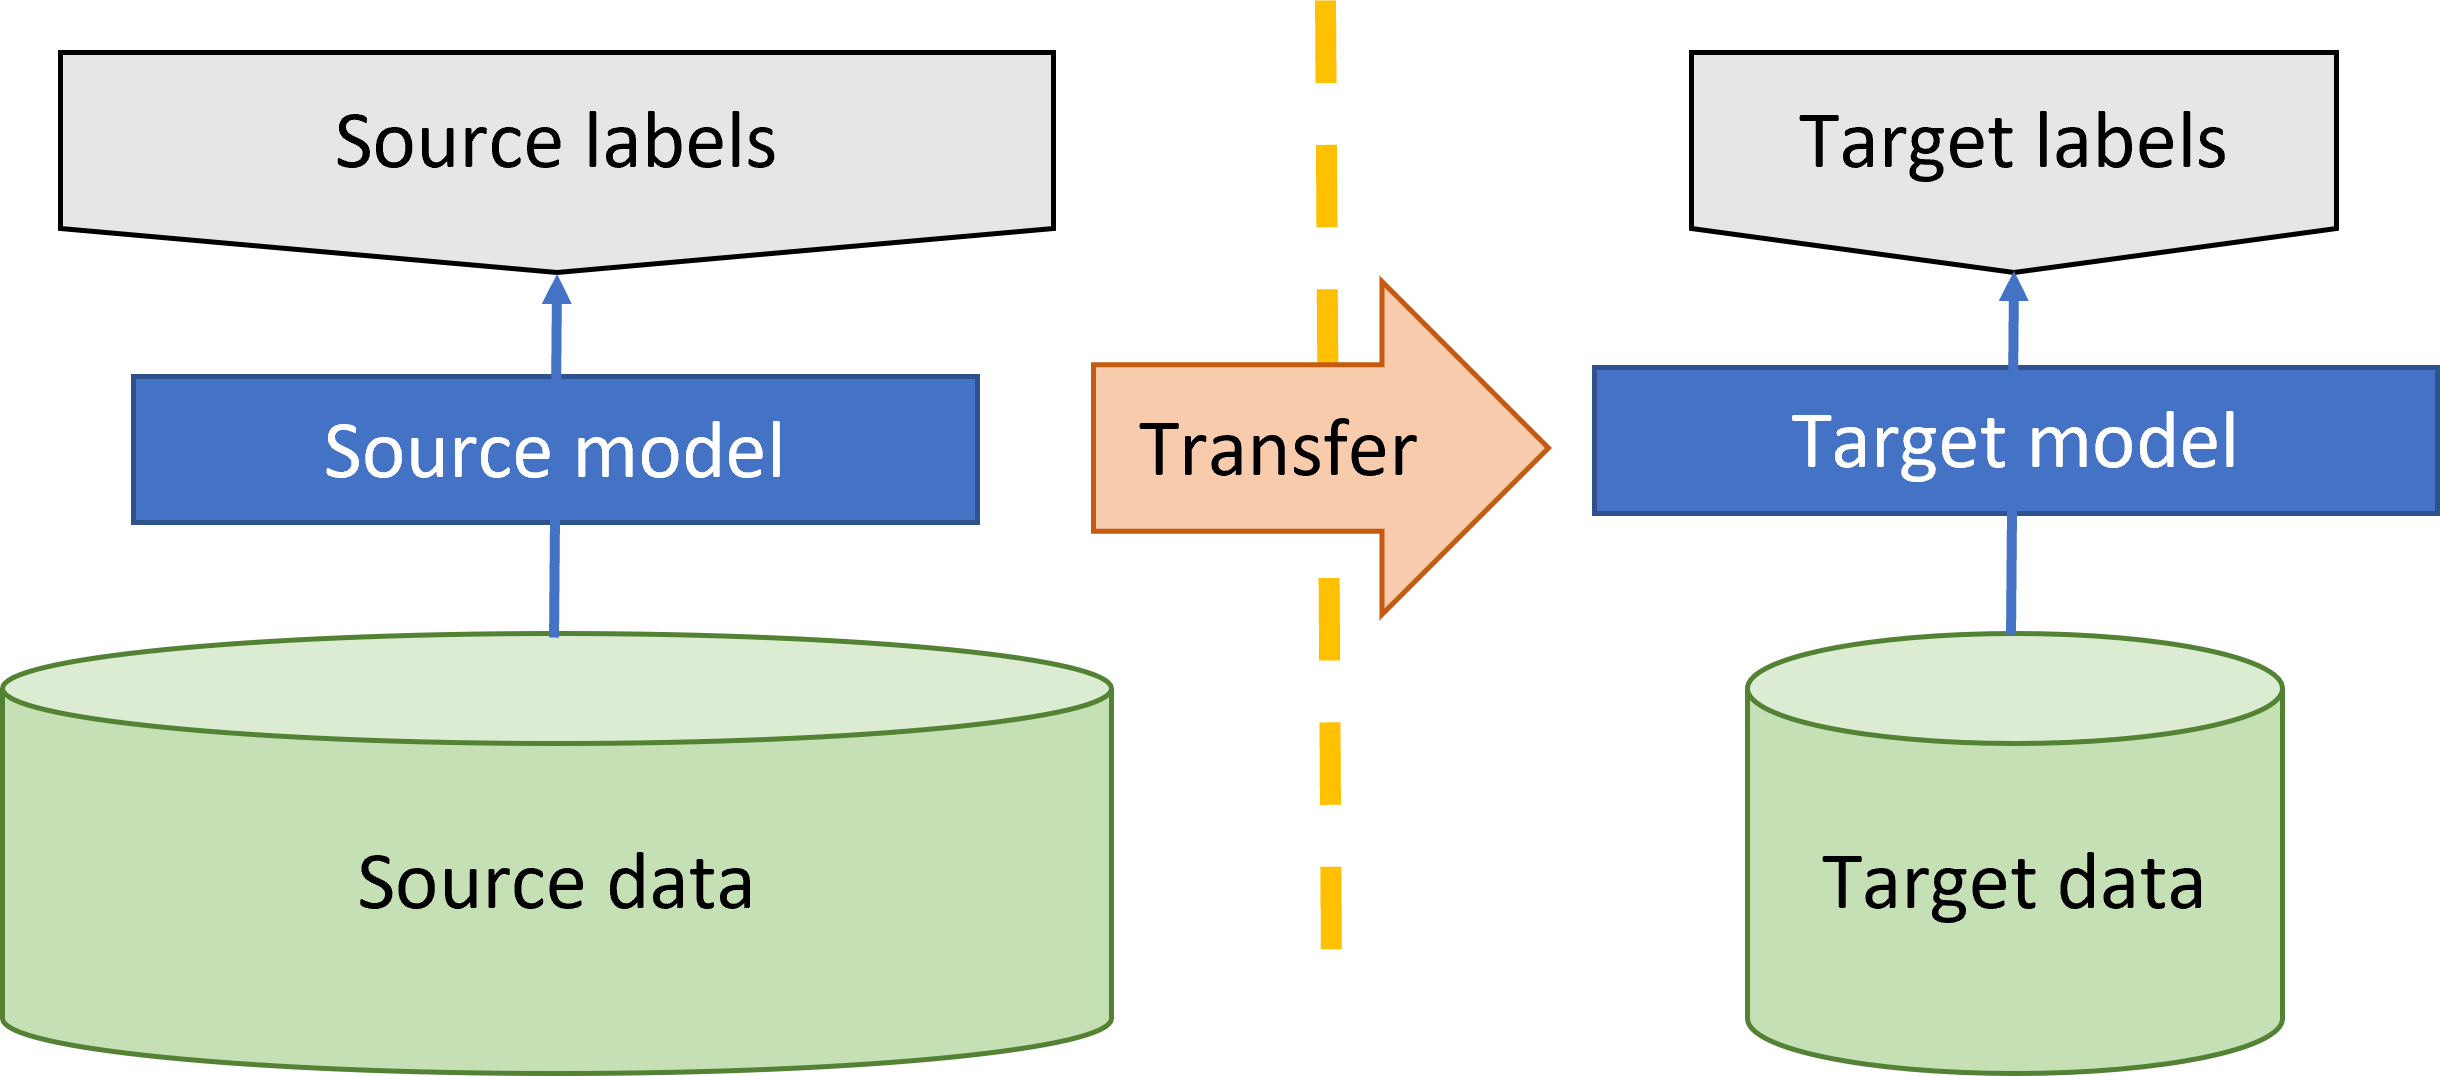
\includegraphics[width=8cm]{Transfer_learning_concept}
		\caption{Concept of transfer learning. Adapted from \protect\cite{Sarkar2018} }
		\label{fig:transferconcept}
	\end{figure} 
	It does so by relaxing the underlying assumption that training and test data for a Machine Learning model should be independent and identically distributed \cite{Weiss2016}. A conceptual picture of transfer learning can be seen in figure \ref{fig:transferconcept}. Although used quite often in different applications \cite{Zhuang2021}, transfer learning concerning environmental sciences has so far mainly been applied in wind farm modelling \shortcite{Hu2016,Qureshi2017}. The concept of transfer learning has not yet been used to improve the precipitation estimation using CML in data-scarce areas. 
		
	Recent research focused on the use of CML data to measure rainfall in tropical regions, more specifically Sri Lanka \shortcite{Overeem2021} and Brazil \shortcite{RiosGaona2017a}. The relatively small amount of reference rain gauges in Sri Lanka especially made this research more challenging compared to well-equipped countries like the Netherlands \shortcite{Overeem2013}. Both of the two studies mentioned above (Sri Lanka and the Netherlands) are based on the PL method. There have not been any efforts yet to analyze the potential of CML for rainfall retrieval using data-driven methods for neither the Netherlands nor Sri Lanka. This research aims to fill this knowledge gap by applying transfer learning of a neural network from Dutch to Sri Lankan CML data.

	
	\section{Research objectives and questions}
	
	The questions asked in this research are the following:
	1) How does a neural network perform on Dutch CML data in retrieving rainfall rates? By training, testing and validating a neural network on the Dutch CML data, this research aims to find out if such a data-driven approach yields better results compared to more traditional approaches.\\
	2) How does transfer learning improve the use of CML in Sri Lanka for measuring precipitation? As transfer learning has the potential to improve the learning curve of a neural network significantly, this question is aimed to find out if applying the concept of transfer learning is useful and worthwhile. Is there a significant benefit to this method that would make it preferable over other more traditional methods?\\
	3) What is the potential of the use of neural networks for 2D interpolation of rainfall maps? A neural network architecture can be used to detect unknown patterns in rainfall distributions and use those to improve the interpolation of rainfall maps. Is this significantly better than the currently used interpolation methods? In other words, is it worth the effort? This question will be dealt with if time allows.\\
		
	\section{Field site and data}
	This research will make use of datasets in two different countries, with a slightly different structure.
	\subsection{The Netherlands}
	The Dutch data used in this research the same as used in previous research \shortcite{Overeem2016}.
	The first research question will make use of the CML data from NEC and NOKIA microwave links, operated by T-Mobile. Both datasets span the period of 14 January 2011 to 30 July 2013, roughly 2,5 years. The data contains 3101 links, but as shown before \shortcite{Overeem2016}, not all of these links will be proven useful or continuously available. The total number of actual links used will therefore be lower, depending on the quality. Received Signal Level (RSL)  is stored at 15-minute intervals, at which the minimum and maximum signal level over the time period are stored. The power resolution of the data is 1 dB (NOKIA) and 0.1 dB (NEC). 
	Apart from the dynamic time signal data, static metadata is included as well. This includes coordinates of the start and end point of the link, distance between these points and frequency per link. Figure \ref{fig:cmlnetworkmaps}a shows the distribution of the links throughout the Netherlands.
	
	As a target dataset, or the reference, a gauge-adjusted radar rainfall dataset is used (freely available as "Radar precipitation climatology" via http://climate4impact.eu) with a resolution of 0.9 km\textsuperscript{2}. The radar is spatially adjusted with the use of both the automated and  manual rain gauge networks operated by KNMI (Royal Dutch Meteorological Institute).
	
	
	\subsection{Sri Lanka}
	The Sri Lankan data is the same as used in previous research \shortcite{Overeem2021}.
	The CML data in Sri Lanka spans 3.5 months (12 September 2012 to 31 December 2012) and similar to the Dutch data, is logged once every 15 minutes (minimum and maximum RSL). The dataset consists of on average 1140 link paths. Static data include start and end point of the link, link length and average frequency. Although the data is available throughout the whole country of Sri Lanka, the network density around the biggest city Colombo is significantly higher, which can be seen in figure \ref{fig:cmlnetworkmaps}b.
	
	
	
	
	\begin{figure*}[h]
		\hspace*{\fill}
		\begin{subfigure}[h]{0.45\textwidth}
			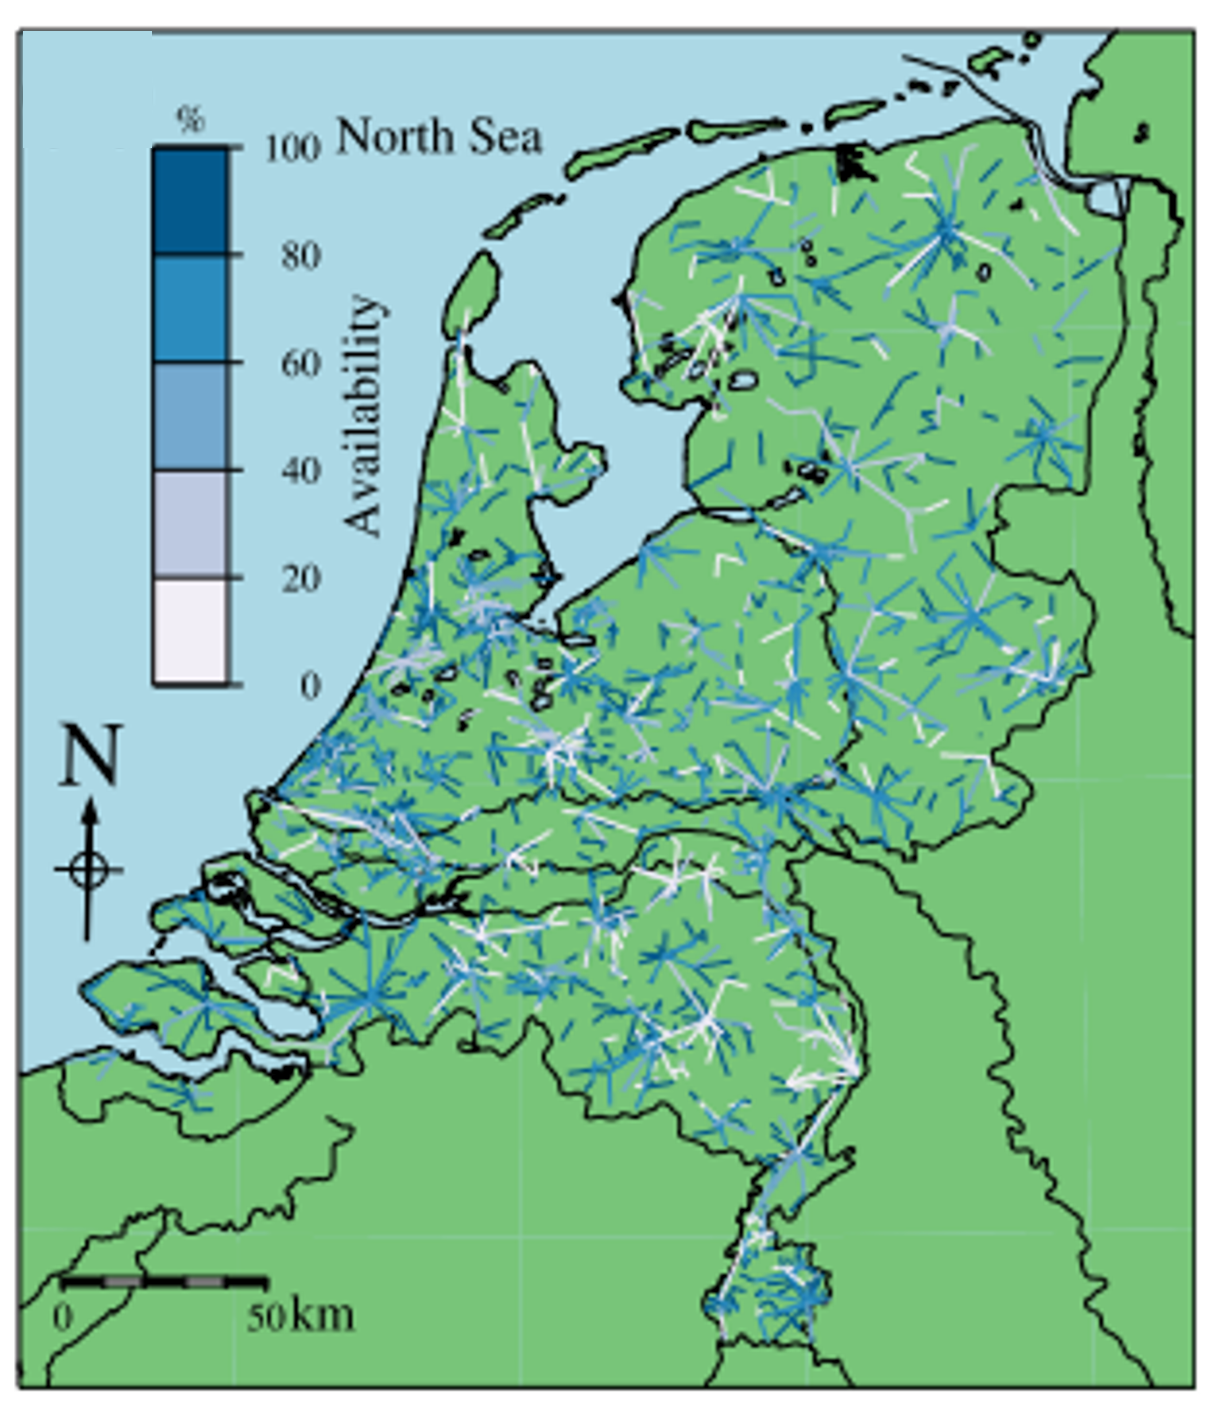
\includegraphics[height= 9cm]{Dutch_CML_network}
			\caption{CML network in the Netherlands. Retrieved from \citeA{Overeem2016}}
		\end{subfigure}
		\hfill%
		\begin{subfigure}[h]{0.45\textwidth}
			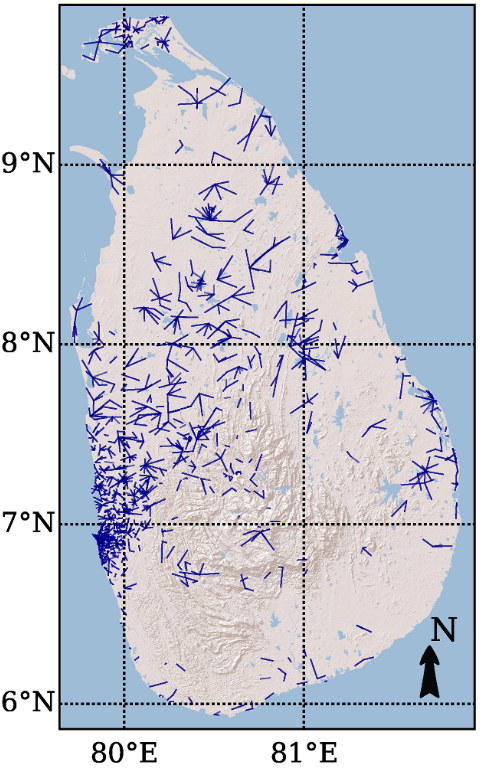
\includegraphics[height=9cm]{SriLanka_CML_network}
			\caption{CML network of Sri Lanka. Retrieved from \citeA{Overeem2021}}
		\end{subfigure}
		\hspace*{\fill}
		\caption{The spatial distribution of the used CML networks}
		\label{fig:cmlnetworkmaps}
	\end{figure*}
	
	The reference dataset consists of manually operated rain gauges, operated by the Sri Lanka Department for Meteorology. Since there are only 36 rain gauges throughout Sri Lanka, a satellite rainfall product will be used to be able to obtain a spatial overview for some precipitation events. Satellite based estimates were retrieved from GPM's combined radar product, as done before by \citeA{Overeem2021}. The precipitation satellite data is freely available (gpm.nasa.gov/data/directory). These satellite based estimates are available roughly once a day, thus not providing a full overview of precipitation but rather an addition to the gauge network. Due to its low temporal resolution, it is not useful as a quantitative reference dataset, but rather serves the purpose of checking the spatial distribution of rain events to get a feeling for the accuracy of the model(s).
	
	\section{Methods}
	\subsection{Neural networks}
	To conduct this research, I will make use of a neural network. Neural networks are part of Machine learning and are structured to mimic the neural structure of the brain. An input signal is transferred through different layers of the network. Every layer consists of different neurons (or nodes). Every node consists of a weighted sum of the complete input signal. The weights that are given to the different values in this input signal, together with a bias that is added to this weighted sum, make up the parameter set of the neuron. 
	The subsequent layers extract combinations out of the previous layer, until finally the network ends up with a prediction with a certain probability. By applying a loss function, the network can learn how to improve, by changing the different parameters in all neurons. By changing these parameters, the model learns to recognize features in the dataset. The to-be-extracted features are unknown beforehand to the researcher. The network itself learns which features are interesting, separable and are helpful in classifying the specific signal. This is the cornerstone of machine learning/deep learning. 
	
	In this research, I will use a Long Short Term Memory (LSTM) architecture as neural network, which is part of the family of Recurrent Neural Networks (RNN). RNN are characterized by the recurrent use of the same bit of network, to keep on improving the prediction. The network typically has one or two layers, depending on the complexity of the features and the signal. The signal is then processed multiple times by the layer(s). RNN are designed for sequential data like the time signals that are used in this research. A disadvantage of RNN is the risk of vanishing or exploding gradients, due to the lack of memory in the network. Without elaborating on the mathematical implementations, vanishing gradients can cause the inability to learn long term dependencies in the data, while exploding gradients can cause the model to crash. LSTM resolve this issue by adding a memory to the model by using different gates to combine old and new data on every recurrent step of the network. The use of LSTM to create a network for CML data has been demonstrated before \shortcite{Habi2019, Diba2021, Pudashine2020}. The networks used in those studies will serve as a source of inspiration for this research. Other types of neural networks have been proposed as well \shortcite{Polz2020}, but as RNN (and specifically LSTM) are designed to work with sequential data, those are preferred in this research.
	
	To obtain the best network for the task, different configurations of hyperparameters are used. These hyperparameters include among others the number of layers within one LSTM cell, the learning rate of the network and the number of evolutions the model passes through.
	
	\subsection{Training, testing and transferring}
	The  Dutch dataset as described in section 3 will be split up in three sets. One is dedicated to training the model, one is used for testing and tuning to different hyperparameter configurations and the final one is for validation. The data will be split in 30\%, 50\% and 20\% for training, testing and validation respectively, in line with \citeA{Polz2020}. The data will be split randomly in order to cover all seasons and timesteps in all subsets. 
	The training data is passed through the LSTM, the loss is calculated for each training sample and the network 'learns' (is updated) by using backward propagation. Backward propagation is a machine learning technique where the final layers are updated first and the updates move backwards through the model. The test dataset will be used to select the best architecture for the model, as different hyperparameters get tested.
	
	After training and testing for a certain number of epochs (evolutions) the model is validated using validation data. The performance on the validation data is the most important and determines the performance of the model overall. 
	
	Once the LSTM is fully trained and its performance is evaluated, transfer learning will be applied, to overhaul the information and knowledge gained by the model to quickly adapt to Sri Lankan data. By removing the last steps before the output probability distribution, the feature extraction part at the basis of the model remains and can be used for a different dataset with different characteristics as well. The use of transfer learning on LSTM models has recently been applied in different fields of research but is still a rather new topic \shortcite{Sagheer2021}. 
	The transferred model will, similarly to the first model, be trained on a subset of the Sri Lankan dataset. Afterwards, it will be tested on the remaining data to evaluate the potential of the transferred model. The model will be validated using the third part of the dataset. 
	
	Finally, both the trained model on the Dutch CML and the transferred model on the Sri Lankan data will be compared to the current performance of CML algorithms \shortcite{Overeem2011, Overeem2021}, which are bundled in the openly available R-package RAINLINK \shortcite{Overeem2016}. During this comparison, focus points will be the overall match with the reference dataset and specifically the performance during periods with rather low or high rainfall rates (top and bottom 20\% of the non-zero rainfall distribution). Low rainfall rates have been a challenge in previous CML research, as the noise in the CML signal is harder to distinguish from small rain-events \shortcite{Uijlenhoet2018}. The performance during periods of higher rainfall is expected to be similar to the PL algorithms performance, as the signal attenuation from large rain-events is quite large and therefore distinguishable. 
	
	\subsection{2-D interpolated rainfall maps}
	Artifical neural networks have been proposed to deal with spatial patterns in rainfall data \cite{Sadeghi2019}. Already 20 years ago, advances have been made in using neural networks for spatial interpolation of environmental variables \cite{Rigol2001}. In this research, a similar neural network structure will be proposed to interpolate the rainfall data obtained from CML. The interpolated map will be compared to a reference map created by using a gauge-adjusted radarproduct.
	These neural networks need terrain information next to the data from the CML. \citeA{Rigol2001} used over 30 different terrain variables to predict a temperature distribution, although most likely a smaller number of variables is needed for the spatial precipitation distribution. Height, distance to the coast and slope/aspect could be relevant terrain parameters, among others.
	The resulting interpolated maps are compared to the more commonly used method of ordinary kriging \shortcite{Overeem2013} to see if the extra effort of using neural networks yields maps that more closely resemble the reference map.
	
	
	\section{Timetable}
	
	Table \ref{tab:schedule} shows the proposed time planning of this research project. Please keep in mind that this planning is preliminary and subject to change. It is still uncertain exactly how challenging the construction and training of the neural networks is. It might take longer than expected. Interpolating using a neural network should be viewed as the bonus part of this reserach that is executed if time allows. If there is some time left, but not enough to tackle the interpolation question well, different research questions concerning the original neural network (and transferred network) will be explored.
	
	
	% table with schedule
	\begin{table*}[t]
		\caption{Schedule of the project.}
		\label{tab:schedule}
		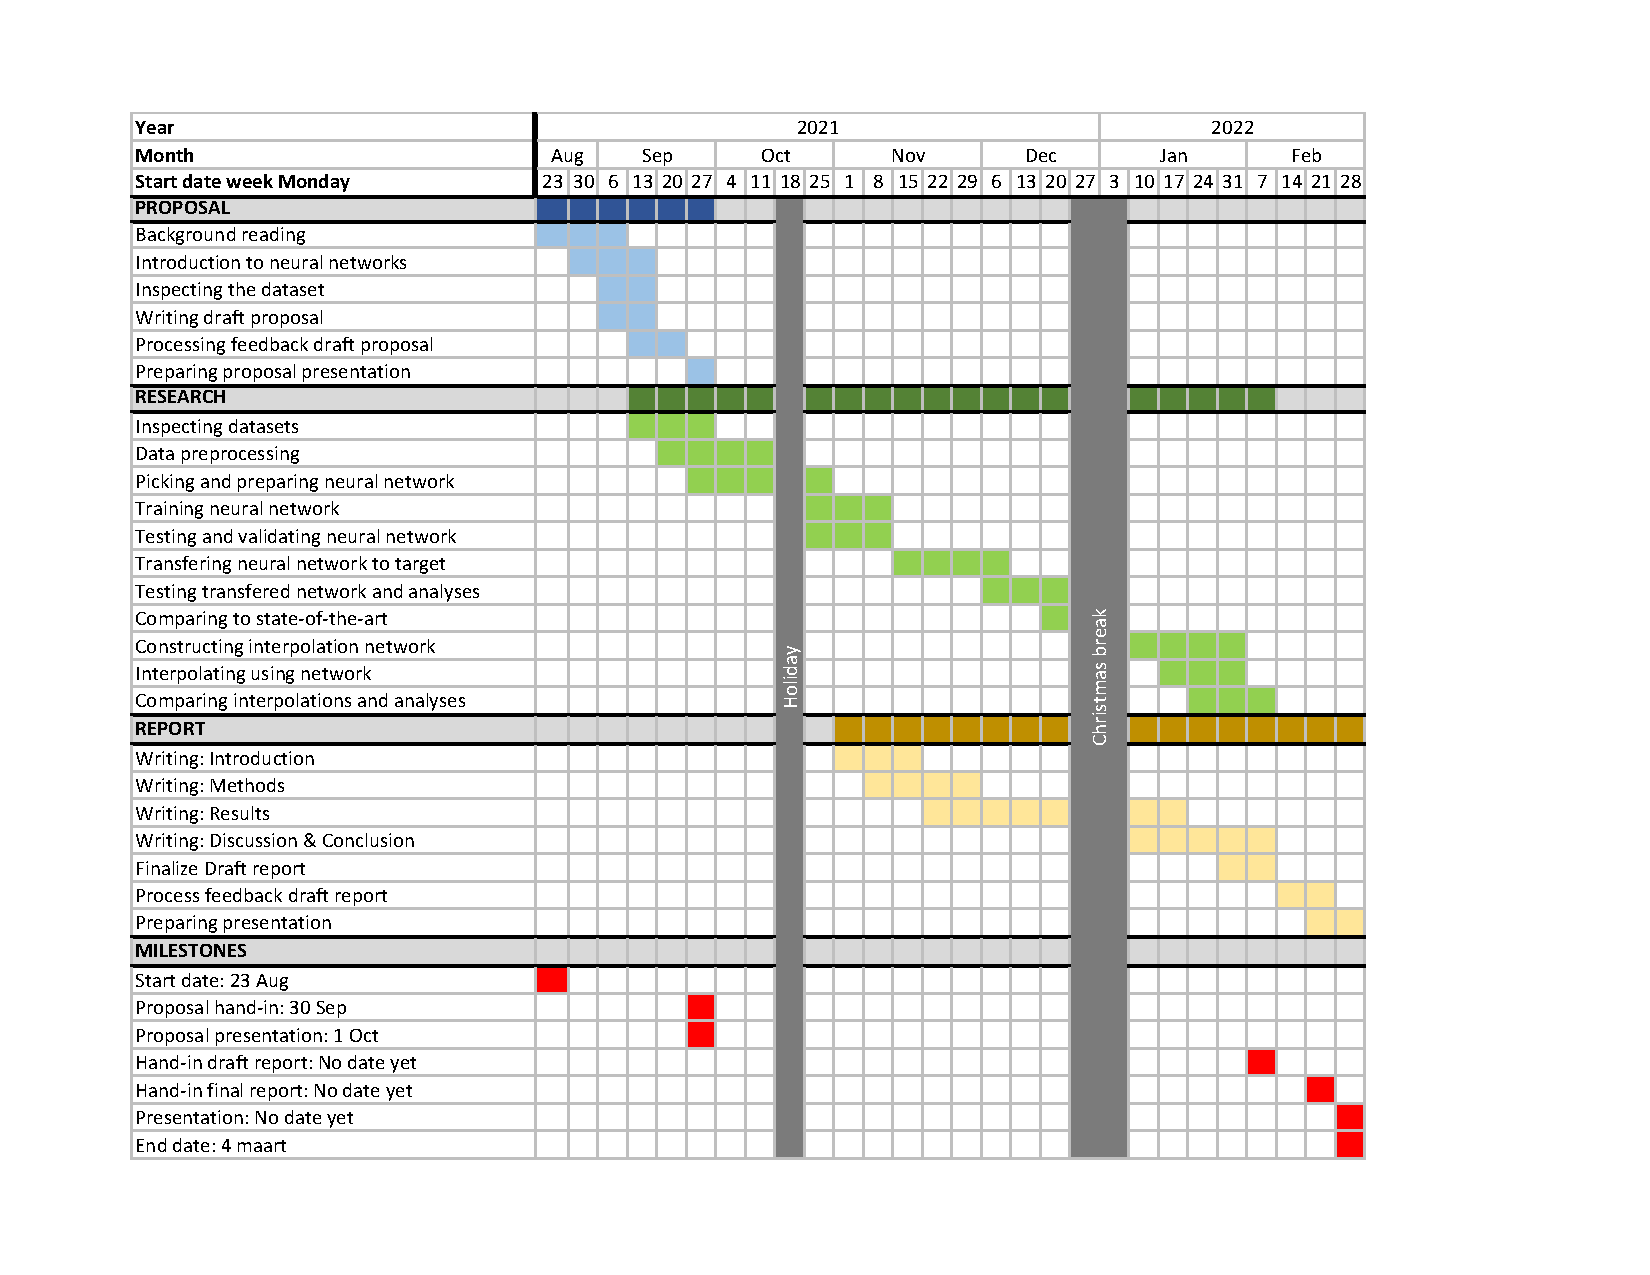
\includegraphics[width=2.1\columnwidth, clip=true]{images/Proposal Schedule.pdf}
	\end{table*}
	% If not the whole table is shown: adjust the numbers behind "trim". 
	% Those are the cropped sides in the order left - bottom - right - top.
	
	
	
	
	%%%%%%%%%%%%%%%%%%%%%%%%%%%%%%%%%
	% BIBLIOGRAPHY
	%%%%%%%%%%%%%%%%%%%%%%%%%%%%%%%%%
	
	% \renewcommand{\bibname}{Bibliography} 
	\bibliographystyle{apacite}
	\bibliography{Proposal_Ludo}
	
	% to add items to the bibliography:
	% option 1. open "references_thesis.bib" in JabRef (free downloadable), enter more papers
	% option 2. open "references_thesis.bib" in NotePad, go to Google Scholar, find paper, click "cite", click "import into BiBTeX", copy text into NotePad
	
	
	
	%%%%%%%%%%%%%%%%%%%%%%%%%%%%%%%%%
	% END
	%%%%%%%%%%%%%%%%%%%%%%%%%%%%%%%%%
	
	
\end{document}

